\chapter{Campo relativista}

	
\begin{tikzpicture}
	\fill [left color=red!50, right color=teal!50] (0,0) rectangle (6.5,.1);
	\fill [left color=teal!50, right color=blue!50] (6.5,0) rectangle (11.5,.1);
	\end{tikzpicture}

\vspace{10mm}
\begin{adjustwidth}{50pt}{50pt}
\begin{ejemplo}
Vamos a seguir construyendo la acción del campo que sea invariante relativista, que cumpla lo que dijo Einstein del espacio-tiempo y también veremos como encontrar la dinámica del campo, lo que nos llevará a las ecuaciones de Euler-Lagrange.
\end{ejemplo}
\end{adjustwidth}
\vspace{5mm}

\section{Acción del campo}

En el capítulo anterior obtuvimos $\ \displaystyle L=\int \dd x \ \dfrac 1 2 \  \partial_\mu \phi \  \partial^\mu \phi $, que, definiendo la 

\begin{definition}

\begin{equation}
\label{T20DensLagran}
\textbf{Desnidad lagrangiana } \qquad \qquad \boldsymbol{ \mathcal L \ = \ \dfrac 1 2 \  \partial_\mu \phi \ \partial^\mu \phi	}
\end{equation}	
\end{definition}

podemos escribir como $\displaystyle \ \ L=\int \dd x \ \mathcal L$

En mecánica clásica, con un número finito de grado de libertad (número finito de partículas, $N< \infty$), tenemos $\ S[q(t)]=\displaystyle \int \dd t L \, \ , $ en nuestro caso, la \textbf{acción de un campo} $\boldsymbol \phi$  se define como: 

$S[\phi]=\displaystyle \int \dd t \ \mathcal L = \int \dd t \int \dd x \ \dfrac 1 2 \  \partial_\mu \phi \  \partial^\mu \phi = \int \int \dd t \ \dd x \ \mathcal L(\phi, \partial_\mu \phi)$

con $\mathcal L=\dfrac 1 2 \left( \partial_0\partial^0 \phi \ + \ \partial_1\partial^1 \phi  \right) = \dfrac 1 2 \left( (\partial_0 \phi)^2 º - \ (\partial_1 \phi)^2 \right)$

\begin{small}\textcolor{gris}{Como la integral es la suma de infinitos puntos, $S\sim
 \displaystyle \sum_{i,j} \mathcal L < \infty$, lo cual impone unas restricciones para el campo, por ejemplo, $\phi(|x|\to \infty)\sim 0$, $\phi(|t|\to \infty)\sim 0$ y también $\partial_0 \phi \to 0$ y $\partial_1 \phi \to 0$ cuando $x,t \to \infty$. Los campos han de cumplir estas exigencias lógicas.}\end{small}
 
 Nuestro espacio-tiempo es de 4 dimensiones ($\mathbb R^3$ espacio, $\mathbb R$ tiempo), por lo que:
 
 $S[\phi]=\displaystyle \int_{-\infty}^{\infty}  \int_{-\infty}^{\infty} \int_{-\infty}^{\infty} \int_{-\infty}^{\infty} \dd t \dd x \dd y \dd z \mathcal L(\phi, \partial_\mu \phi)\, , \ \ $ introduciendo $ct$ por $t$,
 
  $S[\phi]=\displaystyle \int_{-\infty}^{\infty} \int_{-\infty}^{\infty}  \int_{-\infty}^{\infty} \int_{-\infty}^{\infty} c \dd t \ \dd x \ \dd y \ \dd z \ \mathcal L(\phi, \partial_\mu \phi)= \int_{-\infty}^{\infty}
  \int_{-\infty}^{\infty}  \int_{-\infty}^{\infty} \int_{-\infty}^{\infty} \dd x^0 \ \dd x^1 \ \dd x^2 \ \dd x^3 \ \mathcal L(\phi, \partial_\mu \phi) =$
  
  $\displaystyle =\int_{-\infty}^{\infty} \int_{-\infty}^{\infty}  \int_{-\infty}^{\infty} \int_{-\infty}^{\infty} \dd x^4 \ \mathcal L\, , \ $ integral de volumen espacio temporal. Con esto, la definición simplificada de la acción del campo es
 
  \vspace{5mm}  
  \begin{myblock}{Definición simplificada de la acción del campo}
  \begin{large}
  \begin{equation}
  \label{T29DefSimpAccCampo}
  \boldsymbol{S[\phi] \ = \ \int \dd x^4 \ \mathcal L(\phi, \partial_\mu \phi)}	
  \end{equation}
 \end{large}
  \end{myblock}
  
  \vspace{5mm}
  
\section{Dinámica del campo}
\label{T29Funcional}

Para determinar la \emph{dinámica del campo} tenemos que aplicar el \emph{principio de mínima acción}. Hay dos maneras de enfocar esto:

\begin{figure}[H]
	\centering
	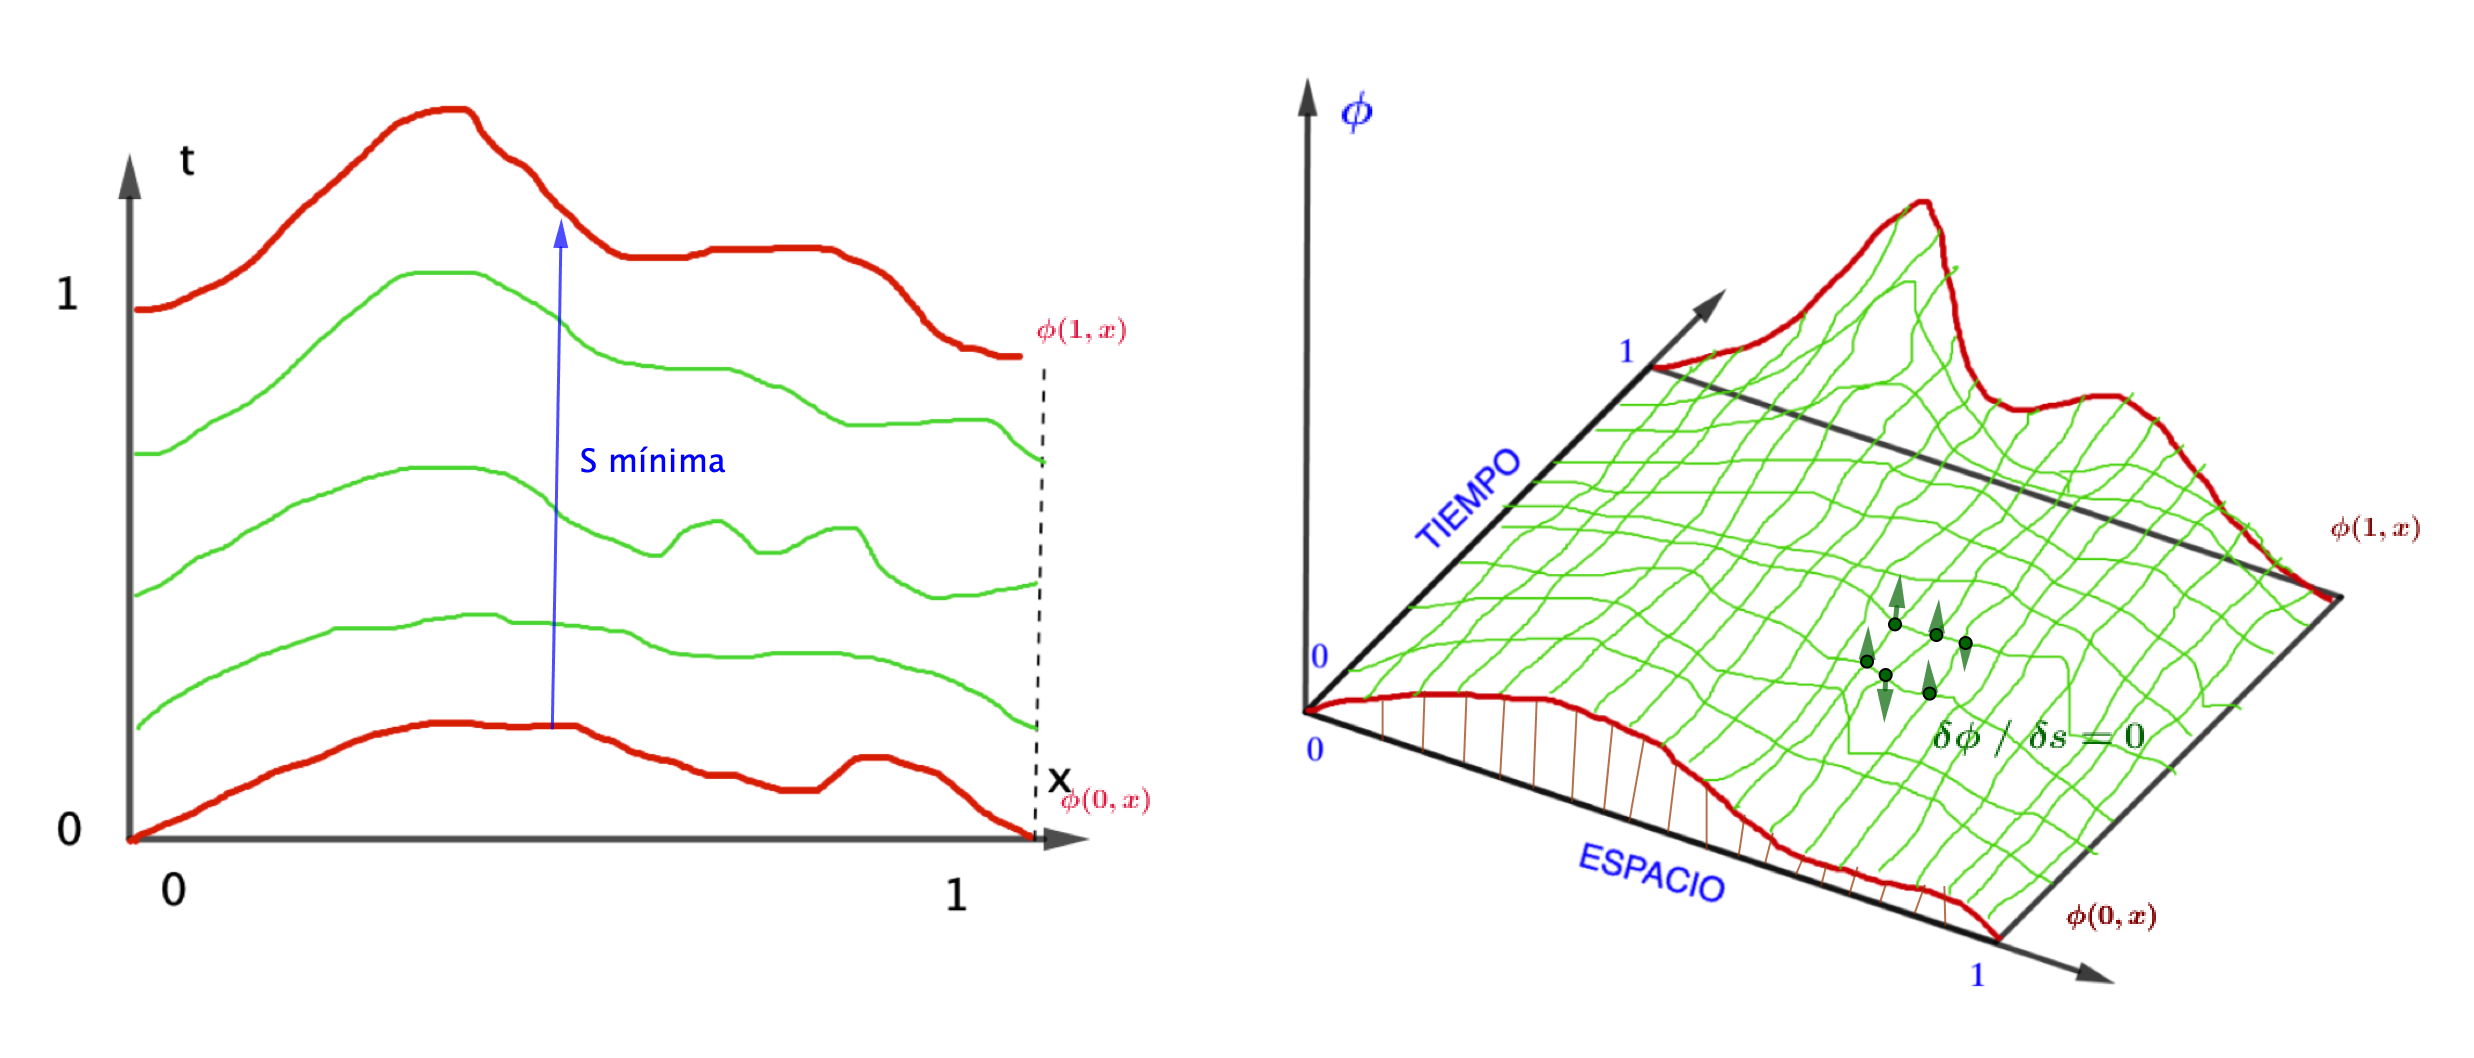
\includegraphics[width=1\textwidth]{imagenes/img29-03.png}
\end{figure}


\begin{enumerate}[$\triangleright\ \ $ a) ]
\item Supongamos que podemos separar el espacio del tiempo, diagrama x-t: (`película')

Imaginemos que podemos separar x-t. Colocándonos en t=0, escogemos el que queremos que sea nuestro campo, $\phi(0,x)$. Si nos colocamos ahora en t=1, queremos que el campo sea $\phi(1,x)$. 

De todas las posibles formas en que la curva  $\phi(0,x)$ se puede convertir en la curva  $\phi(1,x)$, la curva `real' será la que minimice la acción. $\phi(x,t)$ será tal que $s=\displaystyle \int \dd t \int \dd x \ \mathcal L$ sea mínima.

Tenemos como una \textbf{`película'} de curvas posibles desde  $\phi(0,x)$ hasta  $\phi(1,x)$ que minimizarán la acción. 



\item Para generalizar y hablas en abstracto del espacio tiempo, plano x-t: (`sábana')

Ahora no vemos una `película' como en el caso anterior, ahora tenemos la historia completa, en vez de curvas que varían de una a otra, en esta ocasión tenemos una \textbf{`sábana'} en que pasamos del perfil $\phi(0,x)$ al perfil $\phi(1,x)$.


La `sábana' correcta que pasa de uno a otro perfil es aquella cuya acción es mínima. Cada sábana de las múltiples posibles que une los perfiles $\phi(0,x)$ y  $\phi(1,x)$  tiene asociada una acción determinada, un número. La sábana correcta es la que hace que la acción sea mínima.

Para minimizar la acción hacemos que $\delta S=0$. Los puntos de la sábana varían un poco (infinitesimalmente) cada uno de ellos de forma independiente lo que da lugar a una variación infinitesimal del campo, $\delta \phi(t,x)$ en cada punto de la sábana que hará que la variación de la acción sea nula.

Para determinar el campo, el procedimiento es:

$$\delta \phi \ / \ \delta S=0 \quad \to \quad \text{Ecuaciones E-L} \quad \to \quad \text{Ecuación} \quad \to \quad \phi(t,x)$$

Este será el campo que determina la sábana real-verdadera.

\end{enumerate}

Para un sistema mecánico con un número finito de grados de libertad, $N< \infty$, las ecuaciones de E-L son $\ \displaystyle \pdv{L}{q_i(t)}-\dv{t}  \left( \pdv{L}{\dot q_i(t)} \right) = 0$. 

La generalización a un campo es inmediata, $\ q_i(t) \ \to \ \phi(t,x):$

$\displaystyle \pdv{\mathcal L}{\phi} - \dfrac{\partial \mathcal L}{c \partial t}  \left(\displaystyle \pdv{\mathcal L}{ \left( \pdv{\phi}{t} \right) } \right) - 
\pdv{x}  \left(\displaystyle \pdv{\mathcal L}{ \left( \pdv{\phi}{x} \right) } \right) 
- \pdv{y}  \left(\displaystyle \pdv{\mathcal L}{ \left( \pdv{\phi}{y} \right) } \right) 
- \pdv{z}  \left(\displaystyle \pdv{\mathcal L}{ \left( \pdv{\phi}{z} \right) } \right) 
=0\ \ $ \footnote{ Este desarrollo se puede ver con detalle en el capítulo 19 del curso de \emph{Javier Garcia} ``Teoría Cuántica de Campos'', \textcolor{blue}{https://www.youtube.com/c/JavierGarcia110/playlists}} \begin{small} (Ver apéndice \ref{ApendiceFuncional})\end{small}

Las ecuaciones de Euler-Lagrange, usando notación relativista, se pueden expresar en forma simplificada como:

\begin{myblock}{Ec. E-L para el campo}
\begin{large}
\begin{equation}
\label{T29E-L-Campo}
\boldsymbol{
\boxed{ \ 
\pdv{\mathcal L}{\phi} \ - \ \partial_\mu \left( \pdv{\mathcal L}{\partial_\mu \phi} \right) \ = \ 0
}	\ }  \qquad \qquad \mu=0,1,2,3
\end{equation}
\end{large}
\end{myblock}

\vspace{5mm}
Einstein, resumidamente, se dio cuenta de de que las ecuaciones de Maxwell entraban en contradicción con el tema de los observadores inerciales y dijo:  ``\emph{cualquier observador inercial (que se mueva a velocidad constante) debe describir un mismo fenómeno físico con las mismas leyes}'': 
$\ s[\phi]=\int \dd^4 x \ \mathcal L \quad \text{ y } \quad  \pdv{\mathcal L}{\phi}-\partial_\mu \left( \pdv{\L}{\partial_\mu \phi} \right) =0\ $ para determinar el campo $\phi(t,x)$


\begin{multicols}{2}
?`Qué es un observador inercial en nuestro espacio-tiempo, en nuestro plano x-t?

Según Galileo, debe ocurrir que

$\begin{cases}
\ x'=x-vt \\ \ t'=t	
\end{cases}$

Tenemos que comprobar que dos cualesquiera observadores inerciales tienen la misma acción.

	\begin{figure}[H]
	\centering
	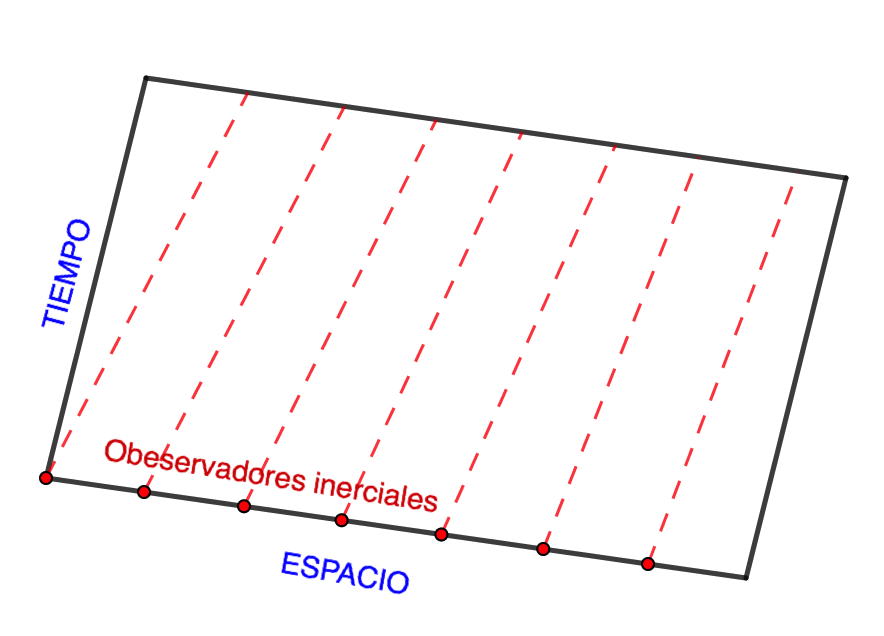
\includegraphics[width=.45\textwidth]{imagenes/img29-04.png}
\end{figure}
\end{multicols}

$S=\displaystyle \int \int \dd t \ \dd x \ \mathcal L = \int \int \dd t \ \dd x \ \dfrac 1 2 \partial_\mu \phi \ \partial^\mu \phi = \int \int \dd t \ \dd x \ \dfrac 1 2 \left[ \left( \pdv{\phi}{t} \right)^2-\left( \pdv{\phi}{x} \right)^2 \right] $

Tomamos $c=1$ por comodidad y hacemos el cambio de coordenadas $\ t,x \to t',x'$

$\triangleright \qquad \displaystyle \pdv{\phi}{t}=
\displaystyle  \cancelto{1}{\pdv{t'}{t}} \pdv{\phi}{t'}+\ \cancelto{-v}{\pdv{x'}{t}}\displaystyle \pdv{\phi}{x'}= \pdv{\phi}{t'}-v\pdv{\phi}{x'}\ = \ \boldsymbol{ \partial_{0'}\phi-v\partial_{1'}\phi \ = \ \partial_0 \phi }$

$\triangleright \qquad \displaystyle 
\pdv{\phi}{x}=
\pdv{\phi}{t'} \cancelto{0}{\pdv{t'}{x'}} + \pdv{\phi}{x'} \cancelto{1}{\pdv{x'}{x}}=
\pdv{\phi}{x'} \ = \ \boldsymbol{ \partial_{1'} x \ = \ \partial_1 x}$

\begin{small}\textcolor{gris}{Transformación inversa de Galileo, $\quad \begin{cases}
\ x=x'+vt=x'+vt' \\ \ \text{ya que } \quad  t'=t	
\end{cases}$} \end{small}

Para el cambio de coordenadas hay que tener el cuenta el determinante del jacobiano:

$\mqty| \displaystyle \pdv{t}{t'} & \displaystyle \pdv{t}{x'} \\ \displaystyle \pdv{x}{t'} & \displaystyle \pdv{x}{x'} | = \mqty| 1 & 0 \\ v & 1 |= 1\, , \ $ luego,

$\displaystyle S=\int \int \dd t' \ \dd x' \ \boldsymbol 1 \ \dfrac 1 2 \left[ (\partial_{0'} \phi - v \partial_{1'} \phi )^2 - (\partial_{1'} \phi)^2 \right]$

$S=\displaystyle
\int \int \dd t' \ \dd x' \  \left[ 
(\partial_{0'} \phi)^2 +v^2 (\partial_{1'} \phi)^2 - 2v \partial_{0'} \phi \partial_{1'} \phi  - (\partial_{1'} \phi)^2 \right]
\quad \boldsymbol{\neq} \quad   
\int \int \dd t \ \dd x \ \dfrac 1 2 \left[ (\partial_0 \phi)^2 - (\partial_1 \phi)^2 \right] $

Luego $\displaystyle
S[t,x]=\int \int \dd t \ \dd x \ \dfrac 1 2 \left[ (\partial_0 \phi)^2 - (\partial_1 \phi)^2 \right]
\quad \boldsymbol{\neq} \quad 
\int \int \dd t' \ \dd x' \ \dfrac 1 2 \left[ ( \partial_{0'} \phi)^2-(\partial_{1'} \phi)^2 \right] =  S(t',x')$

Los observadores inerciales no tendrán las misma leyes, las transformaciones de Galileo no funcionan. Lo que sigue siendo válido es que los observadores inerciales deben tener las misma acción, para ello suponemos que hay otra transformación distinta a la de Galileo, por ejemplo $x'=ax`bt,\ \ t'=dx+ft$ y determinar estas constantes exigiendo que la acción sea la misma para los dos observadores, pero este procedimiento es muy largo.

Como realmente la transformación de Galileo no es del todo falsa, sigue siendo válida para pequeñas velocidades como se comprueba a diario, la \emph{estrategia} a seguir va a ser suponer una transformación de la forma:

$\begin{cases}
\ x'=\gamma(x-vt) \\ \ t'=\gamma \left(t-\dfrac v{c^2} x	 \right)
\end{cases}$, con $\gamma=\gamma(v)$ y el factor $c^2$ responde a necesidades dimensionales.
 
Introduciendo $c$ con $t$, $\quad \begin{cases}
 x'=\ \gamma \left( x-\dfrac v c \ ct \right) \\ \ 	ct'=\gamma \left( ct-\dfrac v{c} x \right)
 \end{cases}$, llamando $\ \beta =\dfrac v c $, tenemos
 $\ \begin{cases}
\ x' \ = \ \gamma \ (x-\beta \ c t )	 \\ \ t' \ = \ \gamma \ (ct - \beta \ x)
\end{cases}$

Usando la notación relativista $x^0=ct$, $\quad \begin{cases} \ x^{1'} \ = \ \gamma \ (x^1-\beta x^0) \\ \ x^{0'} \ = \ \gamma \ (x^0-\beta x^1) \end{cases}$ y continuamos sin saber quién es $\gamma$

Para que esta nueva transformación propuesta reproduzca la transformación de Galileo a bajas velocidades, $\ \boldsymbol{ v<< c \ \Rightarrow \ \beta \to 0 \ \Rightarrow \ \gamma \to 1 }$


------ Para las $x \quad \Rightarrow \beta \to 0 \ \Rightarrow \ x'\approx \gamma \left( x-\dfrac v c c x \right) = \gamma  (x-vt) \ \Rightarrow \ \gamma=1$

------ Para las $t \quad \Rightarrow ct'=\gamma \left( ct - \dfrac v c x \right) \ \Rightarrow \ t'=\gamma \left( t - \cancelto{0}{\dfrac v {c^2}} x \right) \approx \gamma t \ \Rightarrow \gamma = 1\, , \ $ luego

$$\begin{cases}
\ x' \ = \ \gamma \ (x-\beta \ c t )	 \\ \ t' \ = \ \gamma \ (ct - \beta \ x)	
\end{cases}
\qquad \begin{matrix} \beta \to 0 \\ ---\longrightarrow \\ \gamma \to 1 \end{matrix} \qquad
\begin{cases}
\ x'=x-vt \\ \ t'=t		
\end{cases}$$

La transformación propuesta reproduce la transformación de Galileo para bajas velocidades. Ahora tenemos que determinar $\gamma$ exigiendo que esta transformación haga que las leyes de la física sean las mismas para dos observadores inerciales,.

--- $\ \triangleright \quad \displaystyle \pdv{\phi}{x^0}=
\pdv{\phi}{x^{0'}}\pdv{x^{0'}}{x^0}+\pdv{\phi}{x^{1'}}\pdv{x^{1'}}{x^0}=
\pdv{\phi}{x^{0'}} \gamma + \beta \gamma \pdv{\phi}{x^{1'}}$

--- $\ \triangleright \quad $ Análogamente, $\quad \displaystyle \pdv{\phi}{x^1}=
-\beta \gamma \pdv{\phi}{x^{0'}} + \gamma \pdv{\phi}{x^{1'}}$

Elevando al cuadrado y restando, $\quad \displaystyle \left( \pdv{\phi}{x^0} \right)^2 \ - \ \left( \pdv{\phi}{x^1} \right)^2 =
\gamma ^2 \left[ (\partial_{0'} \phi)^2 + \beta^2 (\partial_{1'} \phi)^2 - \left( \beta^2 (\partial_{0'} \phi)^2+ (\partial_{1'} \phi)^2 \right) \right]=$

$=\gamma2 [ (1-\beta^2) (\partial_{0'} \phi)^2 - (1-\beta^2) (\partial_{1'} \phi)^2 ] = \gamma^2 (1-\beta)^2 [(\partial_{0'} \phi)^2 - (\partial_{1'} \phi)^2]=\mathcal L$

Nos falta el jacobiano, $\quad \left|\displaystyle \pdv{x'}{x} \right|=\mqty|\gamma & -\gamma \beta \\ -\gamma \beta & \gamma |=\gamma (1-\beta)^2$

Como $\quad \displaystyle det\left( \pdv{x}{x'} \right) = \dfrac 1 {det \left( \displaystyle \pdv{x'}{x} \right) }\, , \ \ $ tendremos que

$\displaystyle \int \int \dd x^{0'} \ \dd x^{1'} \ \left| \displaystyle \pdv{x}{x'} \right| \ \mathcal L = \int \int \dd x^{0'} \ \dd x^{1'}  \dfrac 1 {\gamma^2 (1-\beta^2)}\gamma^2 (1-\beta^2) [(\partial_{0'} \phi)^2 - (\partial_{1'} \phi)^2] = $

$\displaystyle = \int \int \dd x^{0'} \ \dd x^{1'} \ [(\partial_{0'} \phi)^2 - (\partial_{1'} \phi)^2] \qquad \qquad \forall \gamma$

La acción queda invariante para ambos observadores. 




\begin{multicols}{2}
$\quad$

Estaríamos tentados a sacar la errónea conclusión de que $\gamma$ puede tomar cualquier valor con tal de que $v<<c \Rightarrow \gamma \to 1$ lo cual no es cierto porque además hay que exigir que las leyes de transformación sean las mismas para ambos observadores con tan solo cambiar $\ \beta \leftrightarrow -\beta$ 

	\begin{figure}[H]
	\centering
	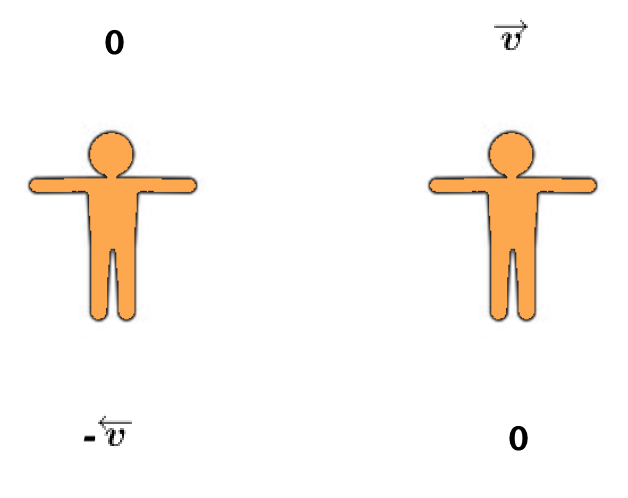
\includegraphics[width=.4\textwidth]{imagenes/img29-05.png}
\end{figure}
\end{multicols}


El resultado de la inversa de la transformación debe ser:

$$\begin{cases}
\ x{1'} \ = \ \gamma \ (x^1-\beta x^0 )	 \\ \ x^{0'} \ = \ \gamma \ (x^0- \beta \ x^1)	
\end{cases}
\qquad \Leftrightarrow \qquad 
\begin{cases}
\ x^1 \ = \ \gamma \ (x^{1'}+\beta \ x^{0'} )	 \\ \ x^0 \ = \ \gamma \ (x^{0'} + \beta \ x^{1'})	
\end{cases}$$

Para que se cumpla esto, se puede demostrar que es necesario que $\quad (1-\beta^2)\gamma^2=1 \, , \ $ es decir,\footnote{ Ver demostración al final del capítulo.}

\begin{equation}
\label{T29gamma}
\boldsymbol{ \subrayado{ \ \boxed  { \ 
\gamma \ = \ + \dfrac{1}{\sqrt{1-\beta^2}}
\ } \ } }	
\end{equation}

El sigo $\ + \ $ garantiza $\ v<< c \ \Rightarrow \ \beta \to 0 \ \Rightarrow \ \gamma \to 1 $
 
\vspace{5mm}
Con esto completamos la deducción de las \textbf{transformaciones de Lorentz} bajo el prisma de la relatividad de Einstein y de imponer que las leyes de la acción sean las mismas para todos los observadores inerciales.
\vspace{5mm}
\begin{myalertblock}{Transformaciones de Lorentz}
\begin{equation}
	\label{T29TLorentz}
\boldsymbol{
\begin{cases}
\ x{1'} \ = \ \gamma \ (x^1-\beta x^0 )	 \\ \\ \ x^{0'} \ = \ \gamma \ (x^0- \beta \ x^1)	
\end{cases}
}		\qquad \qquad \qquad \beta=\dfrac v c \qquad \ \gamma \ = \ + \dfrac{1}{\sqrt{1-\beta^2}}
\end{equation}
\end{myalertblock}


\vspace{10mm}
\begin{ejemplo}
En el próximo capítulo:

Transformación de Lorentz: $\ \to \ (\Delta x^0)^2-(\Delta x^1)^2=(\Delta x^{0'})^2-(\Delta x^{1'})^2\, , \ $ como vio Mimkowski\footnote{``Las ideas sobre el espacio y el tiempo que deseo mostrarles hoy descansan en el suelo firme de la física experimental, en la cual yace su fuerza. Son ideas radicales. Por lo tanto, el espacio y el tiempo por separado están destinados a desvanecerse entre las sombras y tan solo una unión de ambos puede representar la realidad.''}, lo que nos será de ayuda para definir los \emph{cuadrivectores} que nos llevaran al grupo S=(1,3) que será la simetría fundamental de la acción $s[\phi]=\displaystyle \dd^4 x \ \mathcal L(\phi, \partial_\mu \phi)$ con $\mathcal L=\dfrac 1 2 \partial_\mu \phi \partial^\mu \phi$. Toda teoría de campos relativista debe incorporar el grupo de simetría S=(1,3).
\end{ejemplo}


%\vspace{1cm}

\color{NavyBlue}

\begin{center} \rule{200pt}{0.1pt}\end{center}

Demostración de la condición $\ \gamma \ = \ + \dfrac{1}{\sqrt{1-\beta^2}}\ $ al imponer que las transformaciones de Lorentz sean las mismas para ambos observadores inerciales con tal del intercambio $\ \beta \leftrightarrow -\beta$ :

$$\begin{cases}
\ x{1'} \ = \ \gamma \ (x^1-\beta x^0 )	 \\ \ x^{0'} \ = \ \gamma \ (x^0- \beta \ x^1)	
\end{cases}
\qquad \Leftrightarrow \qquad 
\begin{cases}
\ x^1 \ = \ \gamma \ (x^{1'}+\beta \ x^{0'} )	 \\ \ x^0 \ = \ \gamma \ (x^{0'} + \beta \ x^{1'})	
\end{cases}$$

Matricialmente, $\ \mqty(x^{0'}\\ x^{1'})=\mqty(\gamma &-\gamma \beta \\ -\gamma \beta & \gamma ) \mqty(x^0\\x^1) = T \mqty(x^0\\x^1) \ \to \ \mqty(x^0\\x^1)=T^{-1} \mqty(x^{0'}\\x^{1'})$

$|T|=\gamma^2-\gamma^2(1-\beta)^2=\gamma^2(1-\beta)^2 ;\quad T^T=T \quad \to \quad T^{-1}=\dfrac 1{\gamma^2(1-\beta)^2} \mqty(\gamma &\gamma \beta \\ \gamma \beta & \gamma )$

$ \mqty(x^0\\x^1)=T^{-1} \mqty(x^{0'}\\x^{1'})= \dfrac 1{\gamma^2(1-\beta)^2} \mqty(\gamma &\gamma \beta \\ \gamma \beta & \gamma ) \mqty(x^{0'}\\x^{1'})= \dfrac 1{\gamma^2(1-\beta)^2} \mqty( \gamma x^{0'}+\gamma \beta x^{1'} \\ \gamma \beta x^{0'}+\gamma x^{1'} )$

Luego, $\quad \begin{cases}
 \ 	x^0= \dfrac {\gamma x^{0'}}{\gamma^2(1-\beta)^2} + \dfrac {\gamma \beta x^{1'}}{\gamma^2(1-\beta)^2} &\quad = \gamma x^{0'}+\gamma \beta x^{1'} \\
 \ x^1=\dfrac {	\gamma \beta x^{0'}}{\gamma^2(1-\beta)^2} + \dfrac {\gamma x^{1'}}{\gamma^2(1-\beta)^2} &\quad = \gamma \beta x^{0'}+\gamma x^{1'}
 \end{cases} \quad  \leftrightarrow \quad \subrayado{\boldsymbol{\gamma \ = \ + \dfrac{1}{\sqrt{1-\beta^2}}}} \ \qquad\Box$

\color{Black}
\vspace{10mm}

\begin{figure}[H]
	\centering
	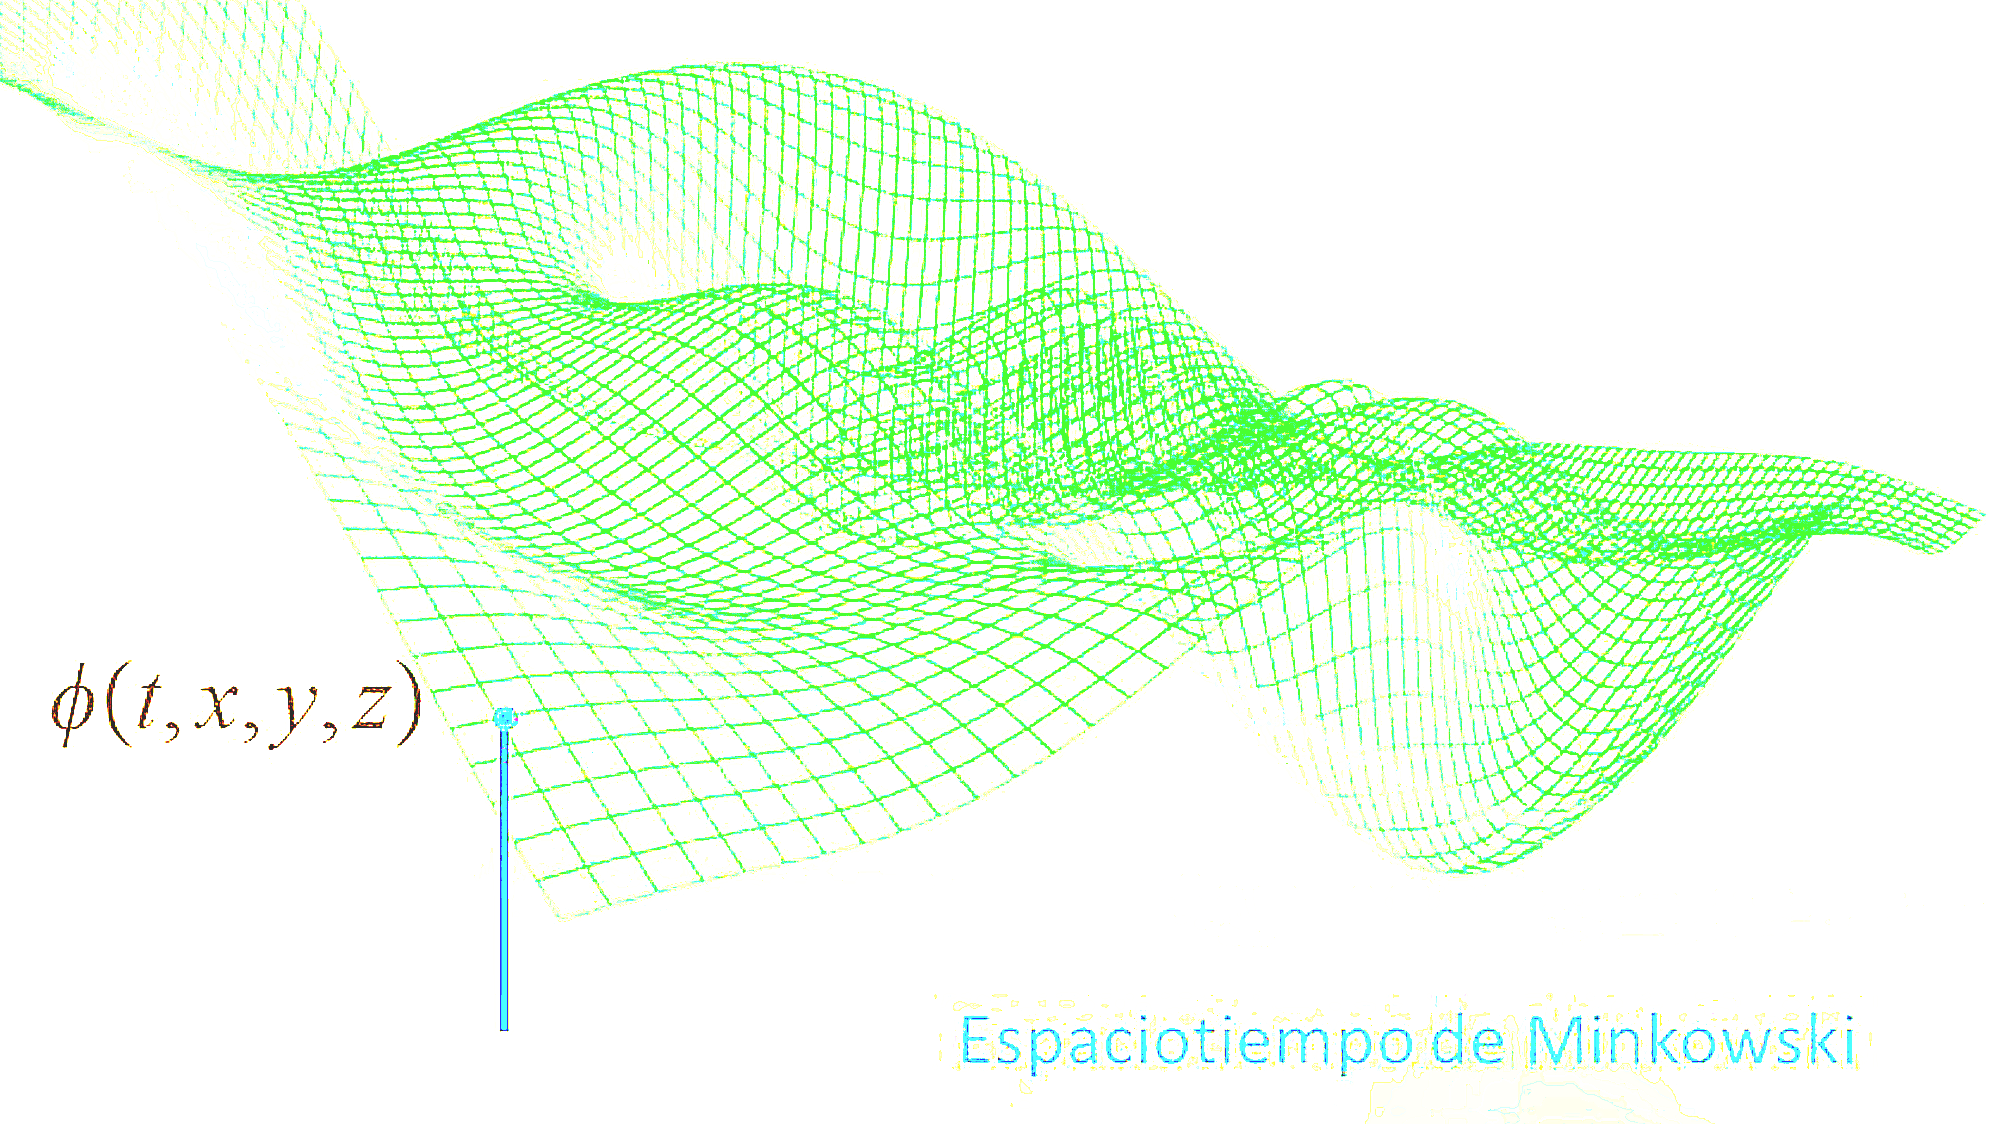
\includegraphics[width=.95\textwidth]{imagenes/img29-06.png}
\end{figure}


